\documentclass[../../main.tex]{subfiles}

\begin{document}

\subsubsection*{Auswertung Fragen zum privaten Umfeld}
\addcontentsline{toc}{subsubsection}{Auswertung Fragen zum privaten Umfeld}

\subparagraph*{Frage: Verwendung von Firewall und Virenscanner}\mbox{}
\begin{figure}[H]
\centering
\framebox[\textwidth]{\scriptsize $n: 259$}
\framebox[\textwidth]{\scalebox{0.9}{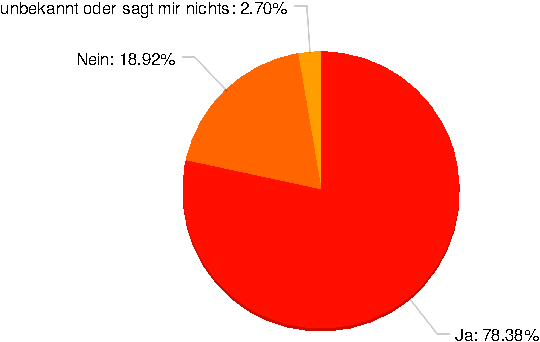
\includegraphics{figures/esurvey/c_pvt_s8_firewall_virus}}}
\caption{Auswertung Frage S8}
\label{S8}
\end{figure}

\subparagraph*{Frage: Automatische Installation von Patches}\mbox{}
\begin{figure}[H]
\centering
\framebox[\textwidth]{\scriptsize $n: 259$}
\framebox[\textwidth]{\scalebox{0.9}{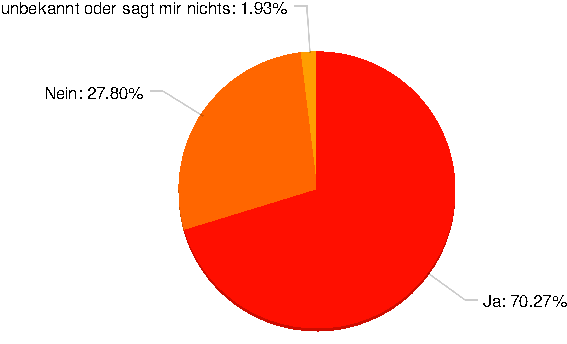
\includegraphics{figures/esurvey/c_pvt_s9_ospatches}}}
\caption{Auswertung Frage S9}
\label{S9}
\end{figure}

\subparagraph*{Frage: Verwendung Administratorenkonto}\mbox{}
\begin{figure}[H]
\centering
\framebox[\textwidth]{\scriptsize $n: 259$}
\framebox[\textwidth]{\scalebox{0.9}{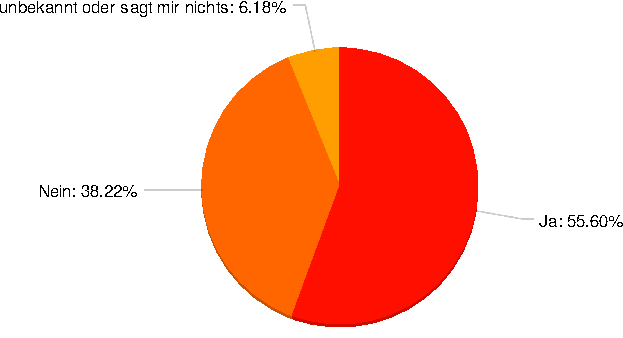
\includegraphics{figures/esurvey/c_pvt_s10_adminaccount}}}
\caption{Auswertung Frage S10}
\label{S10}
\end{figure}

\subparagraph*{Frage: Kann sicheres Passwort erzeugen}\mbox{}

\begin{figure}[H]
\centering
\framebox[\textwidth]{\scriptsize 0 = Trifft überhaupt nicht zu $\vert$ 100 = Trifft voll zu ($n: 259$, $\bar{x}: 86.03$, $\sigma: 18.85$)}
\framebox[\textwidth]{\scalebox{0.9}{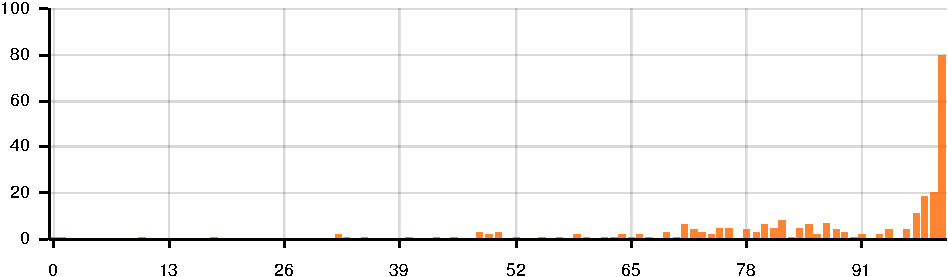
\includegraphics{figures/esurvey/c_pvt_s11_securepwd}}}
\caption{Auswertung Frage S11}
\label{S11}
\end{figure}

\subparagraph*{Frage: Kann Malware auf Computer erkennen}\mbox{}
\begin{figure}[H]
\centering
\framebox[\textwidth]{\scriptsize 0 = Trifft überhaupt nicht zu $\vert$ 100 = Trifft voll zu ($n: 259$, $\bar{x}: 65.20$, $\sigma: 26.88$)}
\framebox[\textwidth]{\scalebox{0.9}{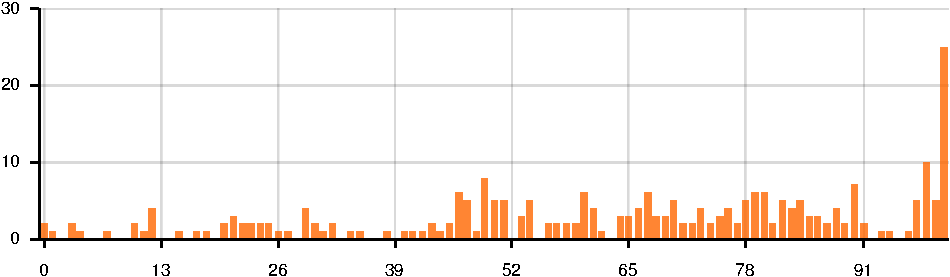
\includegraphics{figures/esurvey/c_pvt_s12_malware_recon}}}
\caption{Auswertung Frage S12}
\label{S12}
\end{figure}

\subparagraph*{Frage: Kann Partner bei Internetbenutzung schützen}\mbox{}
\begin{figure}[H]
\centering
\framebox[\textwidth]{\scriptsize 0 = Trifft überhaupt nicht zu $\vert$ 100 = Trifft voll zu ($n: 260$, $\bar{x}: 66.81$, $\sigma: 27.64$)}
\framebox[\textwidth]{\scalebox{0.9}{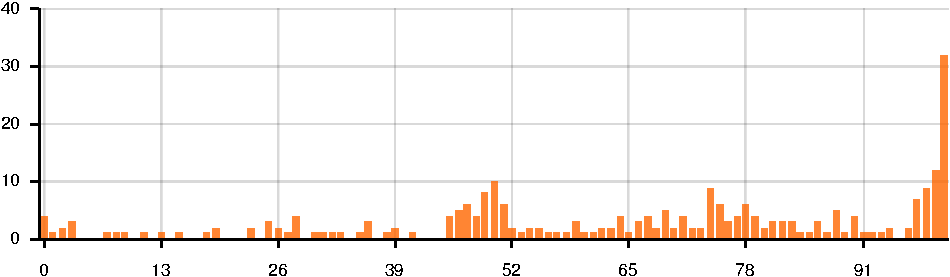
\includegraphics{figures/esurvey/c_pvt_s13_partner}}}
\caption{Auswertung Frage S13}
\label{S13}
\end{figure}

\subparagraph*{Frage: Kann Kinder bei Internetbenutzung schützen}\mbox{}
\begin{figure}[H]
\centering
\framebox[\textwidth]{\scriptsize 0 = Trifft überhaupt nicht zu $\vert$ 100 = Trifft voll zu ($n: 259$, $\bar{x}: 63.69$, $\sigma: 31.10$)}
\framebox[\textwidth]{\scalebox{0.9}{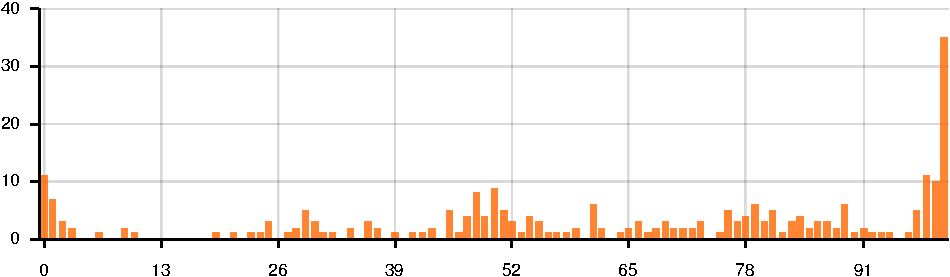
\includegraphics{figures/esurvey/c_pvt_s14_kids}}}
\caption{Auswertung Frage S14}
\label{S14}
\end{figure}

\subparagraph*{Frage: Unterstütze Verwandschaft / Freunde bei Internetbenutzung}\mbox{}
\begin{figure}[H]
\centering
\framebox[\textwidth]{\scriptsize 0 = Trifft überhaupt nicht zu $\vert$ 100 = Trifft voll zu ($n: 259$, $\bar{x}: 64.88$, $\sigma: 30.29$)}
\framebox[\textwidth]{\scalebox{0.9}{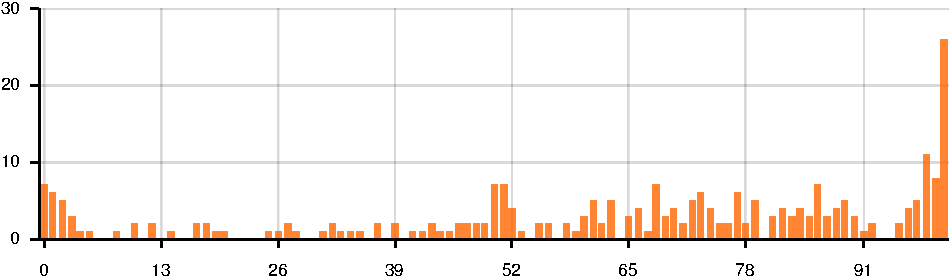
\includegraphics{figures/esurvey/c_pvt_s15_friends_family}}}
\caption{Auswertung Frage S15}
\label{S15}
\end{figure}

\end{document}